\chapter{Motion Detection}
Motion is generally given by a transformation. In video analysis and processing motion is a fundamental feature. 
Motion detection is the process of detecting a change in the position of an object relative to its surroundings or a change in the surroundings relative to an object. We'd like to have an accurate description of objects motion in the scene and camera motion. So we need context in order to understand if is the camera that is moving or it's the object (using displacement vectors).
As before, we're losing information when we're converting a 3D world into a 2D image. So we can't really know if an object is moving or if the camera is moving. We can only know that something is changing in the image.
\\
\[3D: D(X; t_1; t_2) = X' - X = [Dx, Dy, Dz]\]
\[2D: d(x; t_1; t_2) = x' - x = [dx, dy]\]
\\ \textit{NB: x is the projection of X on the image plane.}
\begin{figure}[h]
    \centering
    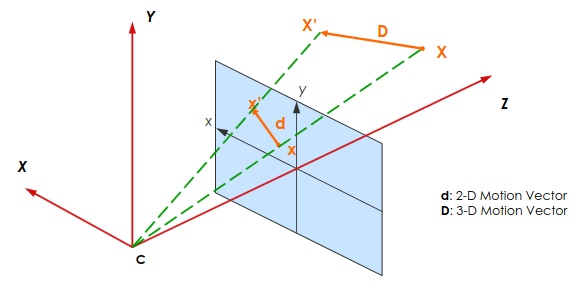
\includegraphics[width=0.7\textwidth]{Figures/2DMotion.png}
    \caption{2D Motion of a 3D object}
\end{figure}
\\We're able to perceive motion only if exist a projection of the image on the image plane. Single camera involves a problem: you can't understand if the point in front of you is growing or coming closer to you.
\\Let's consider an example: 
\begin{figure}[h]
    \centering
    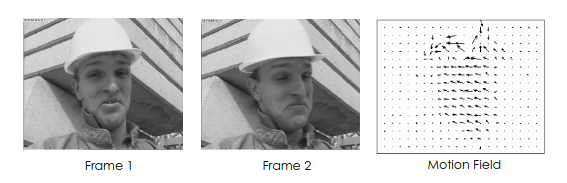
\includegraphics[width=0.7\textwidth]{Figures/Example.png}
\end{figure}
The questions that came up are:
\begin{itemize}
    \item How can I extrapolate the motion field?
    \item Does it really reflect the object displacement?
    \item Is the motion due to the camera or to the object?
\end{itemize}
We can notice an inconsistency in the area of the hat. This is because the hat is a flat surface and the color doesn't allows the window to understand the motion. 
\\\textit{PS: esempio brutale, in una situazione con illuminazione ideale noi, potendo guardare solo una piccola porzione di un foglio bianco, non riusciremmo a capire s eil foglio si sta muovendo oppure no. Il movimento lo cogliamo solo guardando i bordi e la figura del foglio nella sua interezza e nel contesto! per quanto riguarda il cappello immagina di avere tre finestre, o meglio una che slida dentro la parte centrale del cappello, per tutte e tre le finestre ottieni lo stesso risultato quindi niente movimento, o comunque non si capisce un kaiser.}
\\\textbf{2D motion of a rigid object}
\\ The camera is supposed to be fixed, objects move in the 3D space, so motion is generated by a complex combination of arbitrary movements. The 2D projection we obtain is ambiguous because of combinations of different movements can generate the same image. Through an a posterior analysis it’s very difficult to determine the different types of movements that affect the scene.
\section{Motion detection}
Some applications of motion detection are:
\begin{itemize}
    \item Detection
    \item Segmentation
    \item Recognition
    \item Filtering (deblurring, noise suppression)
    \item Compression (transmission and storage)
\end{itemize}
Simplifying the problem, in general, we want to detect changes over time of the image intensity.
This is a  Ill-posed problem, the solution is not unique. (Other problem: lost of 1 dimension, zoom is viewed as a translation)
So the problem is that it doesn't reflect the real motion, where the motion is defined as the velocity $v(x,y,t)$ of the pixels over two consecutive frames.
The motion can be caused by object motion, camera motion and/or illumination changes.
\subsection{Real vs Apparent movement}
2D motion is perceived by changes in the scene over time, but it's not always identify correctly. With a constant illumination, for example, a perfect rotating sphere is perceived as not moving. With an illumination source that rotates around a static sphere, the sphere is perceived as moving.
\subsection{Occlusion}
Occlusion is a problem that arises when a surface is covered/uncovered by the movement of an object.
\begin{figure}[h]
    \centering
    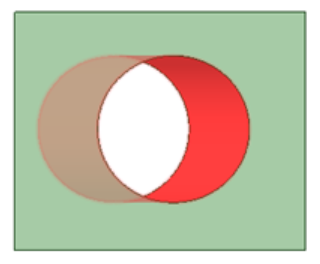
\includegraphics[width=0.5\textwidth]{Figures/Occlusion.png}
    \caption{Occlusion} 
\end{figure}
Now take a look at this example of a circle sliding over a surface. There is a portion of the background (the vivid red one) that will be covered by the circle, and a region(the pale red) that will be uncovered, didn't exist in the previous frame. However, in the end we have notion of movement in this regions but we don't have any information about the white region where nothing seems to be happening. 
\subsection{Aperture}
It's a problem that arises because movement can be detected only along the borders of the objects and only in the direction of the intensity gradient. 
\\\textit{NB: only displacements of the borders are detectable.}
\\To simplify, imagine to drag a paper along its diagonal. We can only see the 2 edges moving up and right but we can't see the actual corner moving.
\begin{figure}[h]
    \centering
    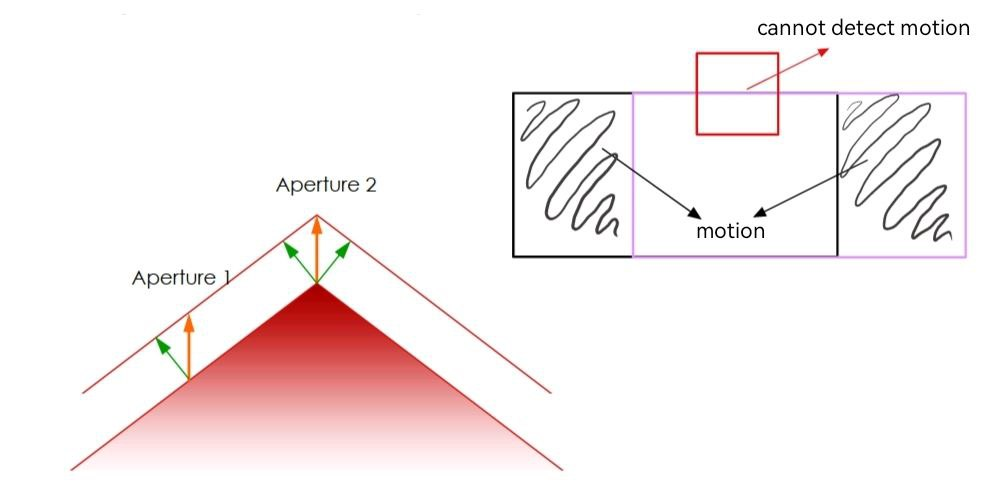
\includegraphics[width=0.7\textwidth]{Figures/Aperture.jpg}
    \caption{Aperture}
\end{figure}
\\TODO: controlla tutta sta parte e modifica l'immagine.
\subsection{Optical Flow}
At this point things look complicated... but we can simplify the problem by making some assumptions:
\begin{itemize}
    \item Object illumination does not change in $[t, t + dt]$;
    \item Distances do not change significantly;
    \item Each point $[x,y]$ is shifted in $[x + dx, y + dy]$.
\end{itemize}
\textit{NB: This is not true in real video but good enough for a first approximation.}
\\\textbf{Optical flow equation}
\\\textit{Hypotesis:} object points keep the same intensity over time\\
\[
    \psi(x,y,t) = \psi(x + dx, y + dy, t + dt)
\]
We can use the Taylor expansion\[f(x + \Delta x) =f(x)+f'(x)\Delta x\] to approximate the function(for small $dx, dy, dz$):
\[
    \psi(x + dx, y + dy, t + dt) \approx \psi(x,y,t) + \frac{\partial \psi}{\partial x}dx + \frac{\partial \psi}{\partial y}dy + \frac{\partial \psi}{\partial t}dt
\]
Comparing the two we obtain that 
\[
    \frac{\partial \psi}{\partial x}dx + \frac{\partial \psi}{\partial y}dy + \frac{\partial \psi}{\partial t}dt = 0
\]
Then, dividing by $dt$ and rearranging the terms we obtain the optical flow equation:
\[
    \frac{\partial \psi}{\partial x}v_x + \frac{\partial \psi}{\partial y}v_y + \frac{\partial \psi}{\partial t} = 0 \quad \text{or} \quad \nabla \psi ^{T} \cdot \mathbf{v} + \frac{\partial \psi}{\partial t} = 0
\]
\textit{PS: if $v=0 \Rightarrow$ we have no variation.}
\\\textbf{Comments:}
\begin{figure}[h]
    \centering
    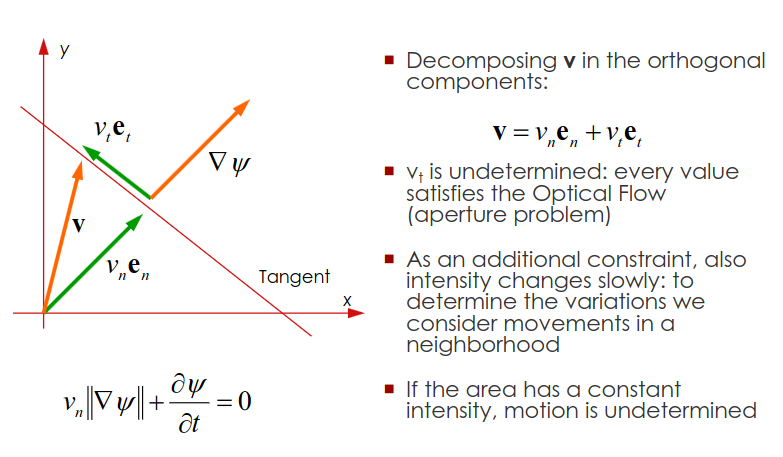
\includegraphics[width=1\textwidth]{Figures/OpticalFlow.png}
    \caption{Optical Flow}
\end{figure}
\section{Motion detection in practice}
We have two possibilities to detect motion: Intensity based and Feature based. However, we have some problems, like the representation of the motion field and the choice of discriminant parameter.
\subsection{Change Detection}
To begin, just take a look at the following example:
\begin{figure}[h]
    \centering
    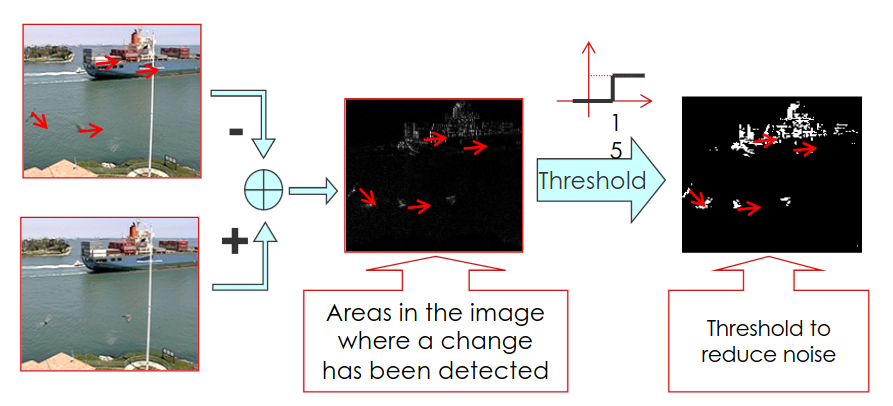
\includegraphics[width=0.7\textwidth]{Figures/ChangeDetection.png}
    \caption{Change Detection}
\end{figure}
\\The two image on the left are the reference image and the current image. We compute the pixelwise subtraction between the two. The result is a binary image, where the white pixels are the pixels that have changed.
\\Looking at the first binary image we can notice a problem, the boat, that is moving, is not detected so well. Indeed, we are not able to understand very well the motion. Our goal is to obtain a motion map that is able to describe the motion field, so the displacement of the pixels.
In this case we choose to change the threshold of the subtraction, so we can obtain a better result. In this way, we reduce noise removing the pixel with loud motion components. Another problem present in both images regards birds. There are two birds flying in the scene but we see four of them. This is due to the fact that the choice of $\Delta t$ is wrong, more specifically is too large. So we need to reduce it increasing the number of samplings.
Another problem that we don't see here but can occur is when we have only one camera and we can't compute correctly the velocity of an object moving in the scene. I'll explain myself better: if there is a car moving on the long diagonal of a rectangle and we have only one camera on the bottom border of the rectangle we probably think, watching the binary image, that the car is moving slower the more it goes away from the camera. 
\\TODO: riscrivi sta parte
\\
\textbf{Formally speaking:}
Change detection is the process of identifying regions in an image that have changed between two or more images. The goal is to obtain a motion map that describes the motion field, i.e. the displacement of the pixels. Can work if the illumination is almost constant.
\\In addition, \underline{frame difference} corresponds to: $I_k - I_{k-1}$
\[
    FD_{k, k-1}(x_1, x_2)= s(x_1, x_2, k)-s(x_1, x_2, k-1)
\]
If FD is non-null, a change has occured. Change can be due to noise, so a threshold is needed to control it:
\[
    z_{k, k-1}(x_1, x_2)= \begin{cases} 1 & \text{if } |FD_{k, k-1}(x_1, x_2)| > \tau \\ 0 & \text{otherwise} \end{cases}
\]
\textit{NB: a good strategy to avoid noise is to use the so-called \underline{cumulative difference.}}
\subsection{Frame differencing}
Is simply subtracting the current image from the previous one. The result is a binary image where the white pixels are the pixels that have changed. A key assumption for this method is that camera must be stationary. The core of this method is to replace background at each frame.
\\For example:
\begin{verbatim}
    B(0) = I(0);
    …
    loop time t
    I(t) = next frame;
    diff = abs[B (t-1) I(t)];
    Map(t) =
    threshold(diff);
    …
    B(t) = I(t);
    end
\end{verbatim} 
Main things to consider are:
\begin{itemize}
    \item Quickly adapts to changes in the background;
    \item Once an objects stops, it is not detected anymore;
    \item Can detect contours of objects;
    \item Only few pixel are usually detected;
    \item If motion is parallel to the edge, then it can lead to artifacts;
    \item By changing the time scale, results can be significantly different.
\end{itemize}
Regarding the last point, we can observe the following:
\[D(N) = ||I(t)-I(t+N)||\]
\begin{figure}[h]
    \begin{subfigure}{0.6\textwidth}
        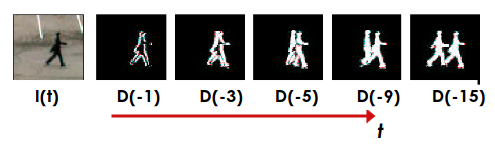
\includegraphics[scale=0.5]{Figures/FrameDifferencing.png} 
    \end{subfigure}
    \begin{subfigure}{0.4\textwidth}
        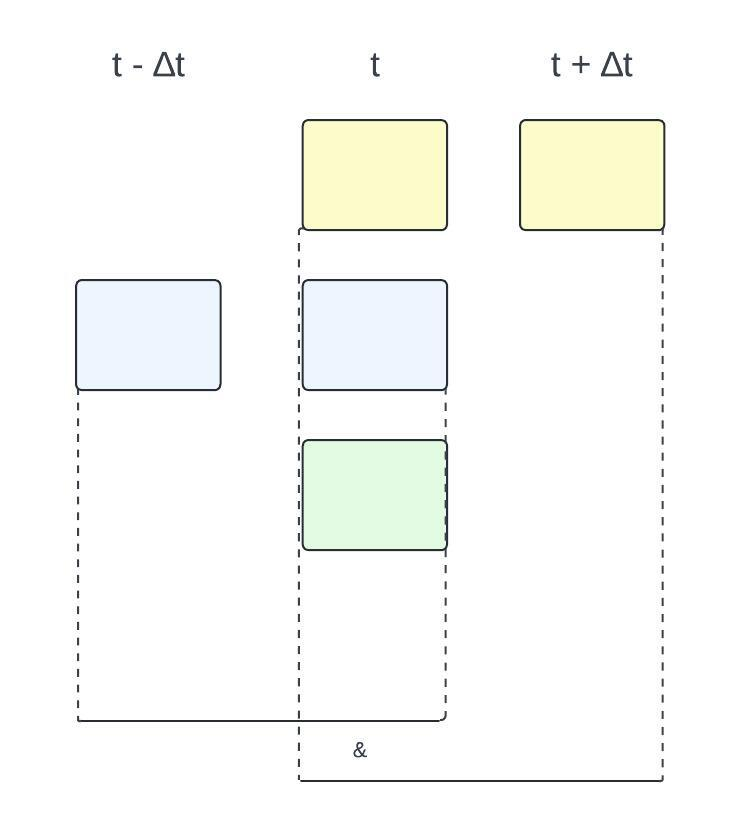
\includegraphics[scale=0.5]{Figures/DifferencingDiagram.jpeg}    \end{subfigure}
        \label{fig:image2}
\end{figure}
The contour of the object becomes clearer, until it doubles: departure and arrival points.
\\\textit{NB: doubling is not good, you can't tell which one is the real one.}
\\Solution $\Rightarrow$ AND between 2 different frames(I understand the real movement).
\subsection{Background subtraction}
Background is modeled as a static image, in general acquired without moving object. The current frame is compared with the background to detect moving objects. The background is updated over time to adapt to changes in the scene.
So, we calculate the difference between current frame and background and assign a label: 1 if it's part of foreground, 0 if it's part of background. 
\\Example: 
\begin{verbatim}
    B = I(0); #initial background
    …
    loop time t
    I(t) = next frame;
    diff = abs[B - I(t)];
    Map(t) =
    threshold(diff);
    …
    end
\end{verbatim} 
\textbf{Comments:}
\begin{itemize}
    \item Good results are obtained if the color of objects differs from the background;
    \item A problem is that if an object enters the scene, it will always be regarded as foreground (aka it won't be detected);
    \item In addition, if a background object moves, both real object and its "ghost" are detected.
    \item It is sensitive to illumination and background changes such as trees, reflections on glossy surfaces like cars and water, shadows, etc.
    \item In addition it is not robust to camera motion.
\end{itemize}
\begin{figure}[h]
    \centering
    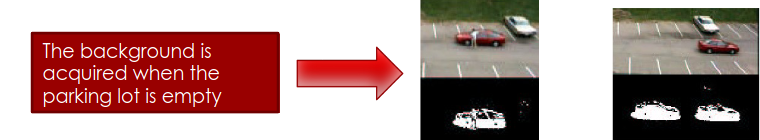
\includegraphics[scale=0.4]{Figures/BackgroundSub.png}
    \caption{Possible problems of Background Subtraction}
\end{figure}
\subsubsection{Adaptive background subtraction}
--TODO: tutto, era un casino e devo ragionarci su.
\subsection{Gaussian average}
The idea is to model the background as a Gaussian distribution. The mean and the variance of the Gaussian are updated at each frame. The current frame is compared with the background model to detect moving objects.
It may use a training sequence to initialize the background model, such as a possibly empty scene.
It take the current pixel value and the previous average and standard deviation. It is very similar to adaptive background subtraction, but more stable.
\[
    \mu_{t} = \alpha I_t + (1-\alpha)\mu_{t-1}
\]
The advantages are its computational efficiency and the low memory requirements.
Pixel goes to foreground if: $|I_t - \mu_t| > k \sigma_t$
Quality depends on a, a depends on the application, a too high value can lead to a slow adaptation to changes, a too low value can lead to a noisy background. Slow update = slow response to changes.
\subsubsection{Improving the Gaussian average}
To improve the Gaussian average we can use a binary operator to update values selectively, so only background values. M=1 if the pixel is foreground and 0 if it's background. This produces a more stable model and prevents pixels from being considered as background when they are not.
\[
    \mu_{t} = M\mu_{t-1} + (1-M)(\alpha I_t + (1-\alpha)\mu_{t-1})
\]
\\\textit{NB: only if you know the situation, perturbations of BG are legit.}
\subsection{Mixture of Gaussians}
With most techniques new objects are sooner or later absorbed in the background. This is because there are changes that appear and disappear faster than the update rate, such as tree leaves, rain, snow, water of a fountain, etc.
It can be that the same pixel represents at different time instants tree leaves and sky/building behind.
The idea is to model the background as a mixture of Gaussians, so using \textbf{K} Gaussian instead of a single one. 
\[
    p(x_t) = \sum_{i=1}^{K} w_{i,t} \mathcal{N}(x_t, \mu_{i,t}, \Sigma_{i,t})
\]
Each of them is used to model a foreground or background object. Theoretical model is complex, we have multi-variate gaussians to model RGB or YUV. In practice we have that components are independent (matrix is diagonal), and variance of each component is the same (\textit{NB: this means that collapse to $\sigma^2$}).  
\\Let's take a deeper look\dots
$w_[i,t] = $ weight for the current Gaussian, $\mu_{i,t} = $ mean for the current Gaussian, $\Sigma_{i,t} = $ variance for the current Gaussian.
Select $K$, rank the Gaussians on the basis of weight, Standard deviation and Peak amplitude.
Hint: the higher the peak and the more compact the distribution (low variance), the more pixel is likely to belong to the background $\Rightarrow$ strong evidence.
Among the $K$ Gaussians, some belongs to the background and some to the foreground. The first $B$ Gaussians are associated to the BG if $\sum_{i=1}^B w_i > T$.
Each incoming pixel is checked against the available models. In case no match is found, a new Gaussian is created. If a match is found (Es a match is found in the pixel is within $(x_t - \mu_{i, t})<2.5\sigma$), the model is updated. If the pixel is not matched with any model, the least probable Gaussian is replaced by the new one centered in $x_t$ with low weight and high variance.  
Also here, update of the weights is necessary: $w_{k,t} = \alpha M_(k,t) + (1-\alpha)w_{k,t-1}$, where $M_(k,t)$ is 1 for the matching model and 0 otherwise (is it's not the matching model, the weight is decreased) and $\alpha$ is still the learning rate. 